\documentclass[12pt]{article}

\usepackage{sbc-template}

\usepackage{graphicx,url}

\usepackage[utf8]{inputenc}  
\usepackage[brazil]{babel}   

\graphicspath{ {./img/} }
     
\sloppy

\title{Estudo Comparativo de Mecanismos de Segurança Aplicados à Autenticação e Autorização em 
Sistemas Web}

\author{Rafael Strack\inst{1}, Adriano Ferrasa\inst{1}}


\address{Departamento de Informática -- Universidade Estadual de Ponta Grossa
  (UEPG)\\
  84.030-900 -- Ponta Grossa -- PR -- Brasil
\email{rafa\_strack@hotmail.com, ferrasa@uepg.br}
}
\begin{document}

\maketitle

\begin{abstract}
  This article presents a comparative study of authentication and authorization mechanisms in web
  systems, aiming to provide an in-depth analysis of the available options and their
  characteristics. The study describes the most commonly used methods such as passwords, tokens,
  multifactor authentication, and OAuth, analyzing their advantages and disadvantages. Additionally,
  sequence diagrams are provided to illustrate the usage flow of each method. Finally, a comparison
  of the studied methods is conducted, evaluating their effectiveness in terms of security. Proper
  understanding of these mechanisms is crucial to ensure the security of web systems and guide the
  correct choice in future projects.
\end{abstract}

\begin{resumo}
  Este artigo apresenta um estudo comparativo dos mecanismos de autenticação e autorização em
  sistemas web, visando fornecer uma análise aprofundada das opções disponíveis e suas
  características. O estudo descreve os métodos mais utilizados, como senhas, tokens, autenticação
  multifator e OAuth, analisando suas vantagens e desvantagens. Além disso, são apresentados
  diagramas de sequência para ilustrar o fluxo de utilização de cada método. Ao final, é
  realizada uma comparação dos métodos estudados, avaliando sua eficácia em termos de segurança. A
  compreensão adequada desses mecanismos é fundamental para garantir a segurança dos sistemas web e
  orientar a escolha correta em projetos futuros.
\end{resumo}


\section{Introdução}

Com a expansão da internet, os sistemas web assumiram um papel crucial no cotidiano de bilhões de
pessoas em todo o mundo. Desde o uso de redes sociais até o gerenciamento de negócios online, essas
ferramentas se tornaram indispensáveis para diversas atividades. Tanto pessoas físicas quanto
empresas dependem desses sistemas para garantir a eficiência e produtividade de suas operações.
No entanto, a segurança desses sistemas é uma preocupação constante para desenvolvedores e
usuários, pois há uma série de ameaças e vulnerabilidades que podem comprometer sua integridade.

A fundação OWASP (\emph{Open Worldwide Application Security Project}) atualiza regularmente um
relatório chamado OWASP Top 10, onde são descritos os 10 riscos de segurança mais críticos em
sistemas web. Na última edição, realizada em 2021, a categoria que ficou em primeira colocação foi
a quebra de controle de acesso. Em sétima colocação, ficou a categoria de falhas de identificação e
autenticação \cite{OWASP2021}. Esses problemas são diretamente relacionados aos processos de
autenticação e autorização de usuários, os quais são essenciais para garantir a proteção adequada
dos sistemas.

De modo geral, a autenticação é o processo de validação de usuários, enquanto a autorização é o
método que fornece as permissões de acesso corretas aos recursos para usuários previamente
autenticados \cite{TUMIN2012}. Atualmente, existem diversos mecanismos de autenticação e autorização
de usuários disponíveis, como senhas, \emph{tokens}, autenticação multifator, OAuth, OpenID, entre
outros. Cada um desses mecanismos apresenta características distintas, pontos positivos e negativos,
sendo fundamental garantir a correta implementação dos mecanismos escolhidos, de forma a assegurar
a efetividade da segurança dos sistemas web.

Diante desse contexto, o presente trabalho tem como objetivo realizar um estudo
comparativo dos diferentes mecanismos de autenticação e autorização, com o propósito
de fornecer uma análise aprofundada que auxilie na escolha adequada desses mecanismos
em projetos de sistemas web. O estudo visa oferecer uma compreensão ampla das
características, pontos fortes e limitações de cada mecanismo, permitindo a seleção
correta e a implementação eficiente das medidas de segurança necessárias.

\section{Autenticação e Autorização}

Na maioria dos sistemas web, é necessário realizar um controle de acesso, para que somente
certos usuários possam acessar recursos protegidos. Para isso, o mecanismo  de controle de
acesso depende de dois processos relacionados: a autenticação e a autorização
\cite{SULLIVAN2011}.

A autenticação pode ser definida como o processo de confirmação de identidade. Em sistemas web,
devido a falta de conhecimento do mundo real, este processo pode não ser simples
\cite{CHAPMAN2012}. Existem três grupos de fatores amplamente utilizados para confirmar a
identidade de um usuário: algo que o usuário sabe, algo que o usuário é e algo que o usuário
possui. No primeiro grupo, inclui-se as senhas, PINs (\emph{Personal Identification Number}) e
frases secretas. No segundo grupo, inclui-se certificados digitais, \emph{smart cards} e
\emph{tokens} de segurança. O terceiro grupo inclui técnicas biométricas, como como impressões
digitais, reconhecimento facial ou de voz, entre outras \cite{SULLIVAN2011}.

% arrumar, complementar, procurar mais referencias sobre a definição de autorização e seus tipos
A autorização é o processo pelo qual o sistema decide se um usuário previamente autenticado
possui permissão para acessar um recurso ou executar uma determinada ação \cite{SPILCA2020}. Ela 
pode ser realizada de várias formas, porém as mais comuns são as baseadas em usuários, garantindo 
acesso aos recursos do sistema web para cada usuário de forma distinta, baseada em perfis 
(\emph{roles}), em que cada usuário possui um perfil, e cada perfil tem diferentes níveis de acesso 
aos recursos do sistema e com o protocolo OAuth \cite{CHAPMAN2012}. Alguns dos métodos de 
autenticação e autorização mais utilizados e conhecidos serão apresentados a seguir.


\subsection{HTTP Basic Authentication}

A HTTP (\emph{Hypertext Transfer Protocol}) Basic Authentication foi definida na especificação
HTTP/1.0 \cite{RFC1945}, porém foi realocada para a RFC 2617 \cite{RFC2617}. Neste tipo de
autenticação, o servidor web recusa uma transação caso o cliente não esteja autenticado,
desafiando-o para obter um nome de usuário e senha válidos. Este desafio de autenticação é iniciado
retornando o status HTTP 401 (não autorizado) e especificando o domínio de segurança
(\emph{security realm}) a ser acessado, com o cabeçalho \texttt{WWW-Authenticate}. Ao receber o 
desafio, onavegador abre uma caixa de diálogo para que o usuário insira as credenciais para acesso 
ao domínio. O navegador então junta as informações de usuário e senha, colocando dois pontos entre 
eles, e os codifica usando o método de codificação base-64. Estas credenciais codificadas são 
colocadas no cabeçalho \texttt{Authorization}, e então a requisição é enviada para o servidor, que 
fará a validação das credenciais e, caso validadas, retorna-se o status HTTP 200 (OK) 
\cite{GOURLEY2002}. Um exemplo do funcionamento deste método de autenticação é mostrado na Figura 
\ref{fig:basicAuth}.

\begin{figure}[ht]
  \centering
  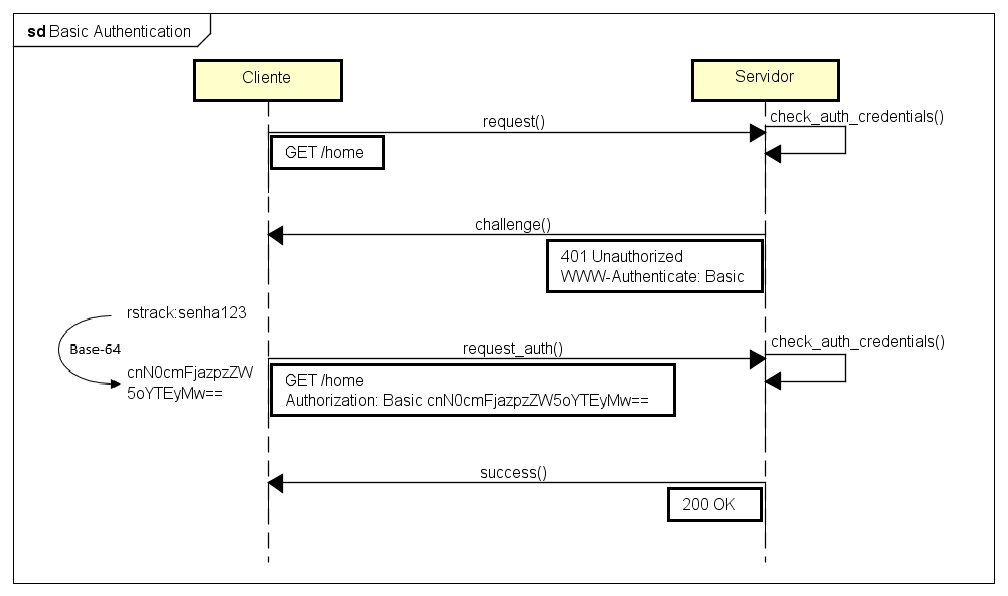
\includegraphics[width=1\textwidth]{Basic Authentication.png}
  \caption{Exemplo de HTTP Basic Authentication}
  \label{fig:basicAuth}
\end{figure}

A diretiva de domínio (\emph{realm}) utilizada nas autenticações HTTP define os espaços de proteção 
do sistema web. Esses domínios permitem que os recursos protegidos sejam particionados, cada um com 
seu próprio esquema de autenticação e/ou autorização \cite{RFC2617}.

A HTTP Basic Authentication é simples e de fácil implementação, porém não possui segurança. As 
credenciais do usuário podem ser facilmente decodificadas, visto que a codificação base64 é 
facilmente reversível, podendo ser realizada em poucos segundos. Também é possível realizar ataques 
de reprodução, visto que terceiros podem capturar pacotes e replicá-los, mesmo que codificados, 
podendo obter acesso ao sistema. Este tipo de autenticação não possui proteção contra \emph{proxies} 
ou \emph{middlewares}, que podem facilmente modificar o corpo da mensagem, e também são vulneráveis 
a servidores falsificados, que se passam por outros para realizar o roubo de credenciais 
\cite{GOURLEY2002}. Além Estes  pontos negativos a autenticação básica não possui encerramento de 
sessão, fazendo com que o usuário  permaneça conectado até o fechamento do navegador.

\subsection{HTTP Digest Authentication}

A HTTP \emph{Digest Authentication} foi especificada na RFC 2019 \cite{RFC2019}, porém também foi 
realocada para a RFC 2617. Foi desenvolvida para ser uma alternativa mais compatível e segura  para 
a Basic Authentication, corrigindo as falhas mais graves da mesma, como a falta de criptografia de 
senhas, vulnerabilidade a captura e reprodução de pacotes contra vários outros tipos comuns de 
ataques \cite{GOURLEY2002}.

Assim como a \emph{Basic Authentication}, a \emph{Digest Authentication} é baseada no paradigma 
desafio-resposta \cite{RFC7616}. A diferença entre estes métodos está nos parâmetros adicionados nos 
cabeçalhos das requisições e respostas. 

O cabeçalho \texttt{WWW-Authenticate} possui a adição de parâmetros para identificação única do 
desafio (\texttt{nonce}), especificação de URLs nas quais a autenticação se aplica 
(\texttt{domain}), identificação da qualidade de proteção concedida pelo servidor (\texttt{qop}) e 
especificação do algoritmo de \emph{hashing} a ser aplicado nas credenciais (\texttt{algorithm}) 
\cite{CHAPMAN2012}. Por padrão, o algoritmo utilizado é o MD5, porém na RFC 7616 foram adicionados 
e recomendados os algoritmos SHA-256 e SHA-512/256 \cite{RFC7616}. Estas funções são de mão única, 
convertendo o valor de entrada em uma condensação de caracteres, sem poder retornar a esse valor a 
partir do resultado.

O cabeçalho \texttt{Authorization} possui a adição de parâmetros para evitar ataques 
\emph{chosen-plaintext} e de repetição (\texttt{nc} e \texttt{cnonce}) \cite{RFC7616}, envio do 
nome do usuário explicitamente, sem nenhuma criptografia (\texttt{username}) e envio da URL de 
forma redundante para verificações de permissão (\texttt{uri}). Os parâmetros \texttt{nonce}, 
\texttt{algorithm} e \texttt{qop} são reenviados neste cabeçalho \cite{CHAPMAN2012}.

%%%%%%%% versão mais extensa, substituída pela versão acima

% Assim como a \emph{Basic Authentication}, a \emph{Digest Authentication} é baseada no paradigma 
% desafio-resposta \cite{RFC7616}. A diferença entre estes métodos está nos parâmetros adicionados 
% nos cabeçalhos das requisições e respostas. O cabeçalho \texttt{WWW-Authenticate} possui a adição os 
% parâmetros \texttt{nonce}, \texttt{algorithm}, \texttt{domain} e \texttt{qop}.

% O parâmetro \texttt{nonce} é um valor único gerado que identifica um desafio. O parâmetro 
% \texttt{algorithm} permite ao servidor especificar o algoritmo de \emph{hashing} a ser aplicado nas 
% credenciais\cite{CHAPMAN2012}. Por padrão, o algoritmo utilizado é o MD5, porém na RFC 7616 foram 
% adicionados e recomendados os algoritmos SHA-256 e SHA-512/256 \cite{RFC7616}. Estas funções são de 
% mão única, convertendo o valor de entrada em uma condensação de caracteres, sem poder retornar a 
% esse valor a partir do resultado. O parâmetro \texttt{domain} serve para especificar a quais URLs a 
% autenticação se aplica. O parâmetro \texttt{qop} indica a qualidade de proteção concedido pelo 
% servidor \cite{CHAPMAN2012}, que pode ser autenticação ou autenticação com proteção de integridade 
% \cite{RFC7616}.

% O cabeçalho \emph{Authorization} recebe como adição os parâmetros \texttt{username}, \texttt{nonce}, 
% \texttt{uri}, \texttt{algorithm}, \texttt{response}, \texttt{qop}, \texttt{nc} e \texttt{cnonce}. O 
% nome de usuário é passado explicitamente, sem nenhuma criptografia. O parâmetro \texttt{uri} é o 
% próprio caminho para o recurso solicitado, enviado redundantemente para o servidor verificar se a 
% solicitação é para um recurso que está dentro da área protegida \cite{CHAPMAN2012}. Os parâmetros 
% \texttt{nc} e \texttt{cnonce} são utilizados para evitar ataques \emph{chosen-plaintext} e de 
% repetição \cite{RFC2617}.

O parâmetro \texttt{response} é a principal parte do cabeçalho \texttt{Authorization}: ele contém 
uma concatenação criptografada de dados no formato \texttt{HA1:nonce:nc:cnonce:qop:HA2}, onde HA1 é 
a concatenação criptografada de \texttt{username}, \texttt{realm} e \texttt{password} e HA2 é a 
concatenação criptografada do método HTTP e da URL da requisição, todos separados por dois pontos 
(:) \cite{CHAPMAN2012}.

O navegador faz todo o cálculo resultante no valor de \texttt{response}. O servidor, que possui 
todos os valores necessários para este cálculo, também o faz e compara com o valor recebido. Caso 
as credenciais sejam válidas, retorna-se o status HTTP 200 (OK) e o cabeçalho 
\texttt{Authentication-Info}. Este cabeçalho contém parâmetros utilizados para uma futura 
autenticação (\texttt{nextonce}), para autenticação mútua (\texttt{rspauth}) e possui o reenvio dos 
parâmetros \texttt{qop}, \texttt{cnonce} e \texttt{nc}. Um exemplo do funcionamento deste método de 
autenticação é mostrado na Figura \ref{fig:digestAuth}.

\begin{figure}[ht]
  \centering
  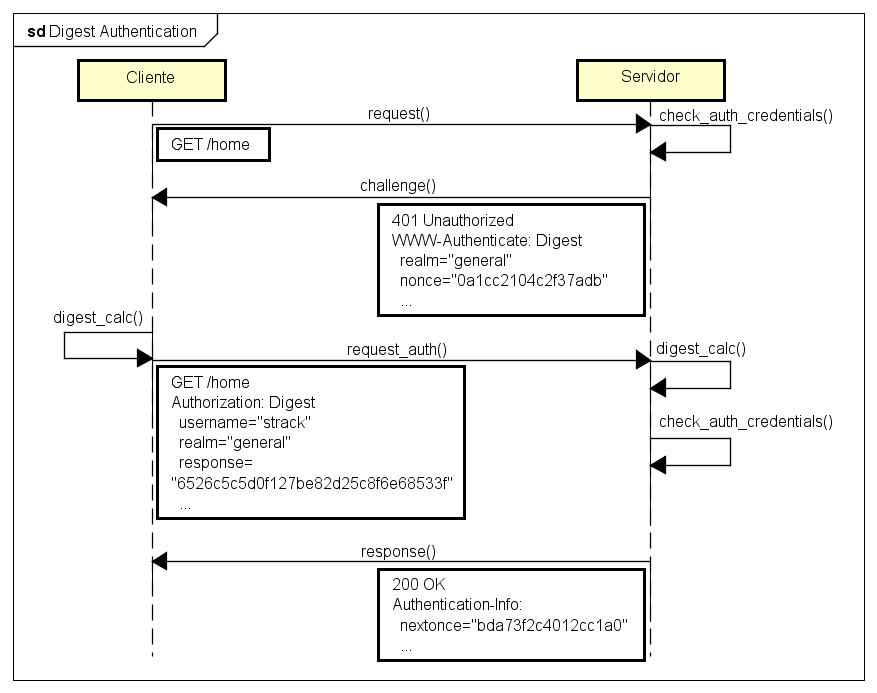
\includegraphics[width=1\textwidth]{Digest Authentication (Simplified).png}
  \caption{Exemplo de HTTP Digest Authentication}
  \label{fig:digestAuth}
\end{figure}

Apesar da grande melhora de segurança em relação a \emph{Basic Authentication}, este método possui 
diversos riscos de segurança. Os cabeçalhos \texttt{WWW-Authenticate} e \texttt{Authorization} 
possuem certo nível de proteção a manipulação, porém os outros não. Se valores de \texttt{nonce} 
não forem exclusivos para cada transação, ataques de repetição poderão ser realizados. Se não for 
estabelecida nenhuma política de força de senha, poderão ser realizados ataques de dicionário, 
tentando adivinhar a senha e o \texttt{nonce}, visto que o nome do usuário é obtido sem esforço.
Se a requisição passar por \emph{proxies} hostis ou comprometidos, o cliente pode ficar vulnerável 
a ataques \emph{man-in-the-middle} \cite{GOURLEY2002}. O encerramento de sessão também não foi 
implementado neste método de autenticação.

\

\subsection{Session-Based Authentication}
\
\subsection{Token-Based Authentication}
\
\subsection{OAuth e OAuth2}
\
\subsection{OpenID}
\
\section{Materiais e Métodos}
\
\section{Resultados e Discussão}
\
\section{Conclusão}
\
% \section{First Page} \label{sec:firstpage}

% The first page must display the paper title, the name and address of the
% authors, the abstract in English and ``resumo'' in Portuguese (``resumos'' are
% required only for papers written in Portuguese). The title must be centered
% over the whole page, in 16 point boldface font and with 12 points of space
% before itself. Author names must be centered in 12 point font, bold, all of
% them disposed in the same line, separated by commas and with 12 points of
% space after the title. Addresses must be centered in 12 point font, also with
% 12 points of space after the authors' names. E-mail addresses should be
% written using font Courier New, 10 point nominal size, with 6 points of space
% before and 6 points of space after.

% The abstract and ``resumo'' (if is the case) must be in 12 point Times font,
% indented 0.8cm on both sides. The word \textbf{Abstract} and \textbf{Resumo},
% should be written in boldface and must precede the text.

% \section{CD-ROMs and Printed Proceedings}

% In some conferences, the papers are published on CD-ROM while only the
% abstract is published in the printed Proceedings. In this case, authors are
% invited to prepare two final versions of the paper. One, complete, to be
% published on the CD and the other, containing only the first page, with
% abstract and ``resumo'' (for papers in Portuguese).

% \section{Sections and Paragraphs}

% Section titles must be in boldface, 13pt, flush left. There should be an extra
% 12 pt of space before each title. Section numbering is optional. The first
% paragraph of each section should not be indented, while the first lines of
% subsequent paragraphs should be indented by 1.27 cm.

% \subsection{Subsections}

% The subsection titles must be in boldface, 12pt, flush left.

% \section{Figures and Captions}\label{sec:figs}


% Figure and table captions should be centered if less than one line, otherwise justified and 
% indented by 0.8cm on
% both margins, as shown in Figure. The caption font must
% be Helvetica, 10 point, boldface, with 6 points of space before and after each
% caption.


% In tables, try to avoid the use of colored or shaded backgrounds, and avoid
% thick, doubled, or unnecessary framing lines. When reporting empirical data,
% do not use more decimal digits than warranted by their precision and
% reproducibility. Table caption must be placed before the table (see Table 1)
% and the font used must also be Helvetica, 10 point, boldface, with 6 points of
% space before and after each caption.

% \section{Images}

% All images and illustrations should be in black-and-white, or gray tones,
% excepting for the papers that will be electronically available (on CD-ROMs,
% internet, etc.). The image resolution on paper should be about 600 dpi for
% black-and-white images, and 150-300 dpi for grayscale images.  Do not include
% images with excessive resolution, as they may take hours to print, without any
% visible difference in the result. 

% \section{References}


% The references must be listed using 12 point font size, with 6 points of space
% before each reference. The first line of each reference should not be
% indented, while the subsequent should be indented by 0.5 cm.

\bibliographystyle{sbc}
\bibliography{references}

\end{document}
